
\begin{figure}[tbhp]
        \centering
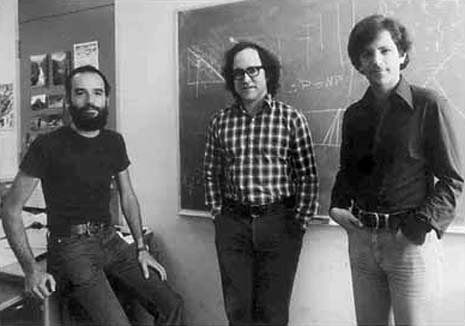
\includegraphics[width=0.75\textwidth]{./images/rsa.jpeg}
        \caption{Adi Shamir, Ronald Rivest, and Leonard Adelman}\label{fig:rsa}
\end{figure}

\section{RSA Algorithm}
\epigraphwidth=0.4\textwidth
\epigraph{\emph{The magic words are \emph{Squeamish Ossifrage}.}}{---Ronald L. Rivest}

\noindent The security of RSA relies on the practical difficulty of
factoring the product of two large prime numbers, known as the
\emph{factoring problem}. Breaking RSA encryption is known as the
\emph{RSA problem}. Whether it is as difficult as the factoring problem
is an open question. There are no published methods to defeat the system
if a large enough key is used, but RSA would be vulnerable to attack by
a \emph{quantum computer}.

RSA involves a public key and a private key. Everyone can know the
public key, and it is used for encrypting messages. The intention is
that messages encrypted with the public key can only be decrypted by
using the private key. The integers $n$ and $e$ represent the public
key. The private key is represented by the integer $d$.

The public key consists of the modulus $n$ and the public exponent $e$.
The private key consists of the private exponent $d$, which must be kept
secret; $p$, $q$, and $\varphi(n)$ must also be kept secret since they
are used to calculate $d$. In fact, $p$ and $q$ ($\varphi(n)$ is
calculated from them) can be discarded after $d$ has been computed.

We proceed by choosing two large random primes $p$ and $q$, these
numbers must be kept secret. We then publish the number $n = p q$. You
might wonder why we can do this, and the reason is that it is
\emph{believed} to be hard to factor large composite integers into their
constituent primes. The \emph{fundamental theorem of arithmetic} tells
us that every integer has a \emph{unique} prime factorization.

Choose a \emph{random} integer $2 < e < n \ni \gcd(e, \varphi(n)) = 1$,
where $\varphi(n) = (p-1)(q-1)$. $\gcd(a, b)$ indicates the greatest
common divisor of $a$ and $b$, which is commonly computed using Euclid's
algorithm, which is defined recursively as:
\[
\gcd(a, b) =
\begin{cases}
         a  & \text{if}\; a = b \\
         \gcd(a, b - a)  & \text{if}\; a < b \\
         \gcd(a - b, b) & \text{if}\; a > b \
\end{cases}
\]
though we can calculate it much more rapidly using division. A good
choice for $e$ is $2^{16} + 1 = 65537$. You will understand why---to
some extent---after you finish \S \ref{numthm}.
Here's a hint: How many $1$ bits are in that number?

The $\varphi$ function is called the \emph{totient} of $n$, and that
denotes the number of positive integers up to a given integer $n$ that
are relatively prime to $n$. Note that for any prime $p$, $\varphi(p) =
p - 1$, and so $\varphi(n) = \varphi(p q) = (p-1)(q-1)$. We can share
$e$ with impunity. We say that our \emph{public key} is the pair
$\langle e, n \rangle$.

We now calculate a unique secret integer $d\in \{0, \ldots, n-1\}$ such
that $d \times e \equiv 1 \pmod{\varphi(n)}$. How do we find this $d$?
It turns out that we have known how to do it for more than $2300$
years---we use an algorithm attributed to \emph{Euclid}. How is it that
we can easily calculate $d$ while our adversary cannot? We know a secret
that he does not: we know $\varphi(n)$ while he only knows $n$. We call
$d$ our \emph{private key}.

We now define two functions: $D(m) = m^e \pmod{n}$ and $E(c) = c^d
\pmod{n}$. We will show in \S\ref{proof} that $\forall m \in \{0,
\ldots, n-1\}$ that $D(E(m)) = E(D(m)) = m$. Since $D$ and $E$ are
\emph{mutual inverses} and this will enable us to perform not only
encryption but also digital signatures.
